\section{Bounded Material Extension: Wood}
\subsection{Population and unchanged intervention}
The wood extension asks whether the corrected-minus-raw contrast has the same direction beyond ordinary plastic, not whether wood performance can be improved by further tuning. Before new inference or scoring, we audited the historical 116-image wood panel. The shared Replay teacher used six wood-day images (23 corners) in recording REC\_001 and three plastic-night images (15 corners) in REC\_002. The latter recording also contains wood-night frames, despite different session names. We excluded all 71 evaluation images from these two teacher-exposed recordings, not just the five exact teacher-image overlaps. The fixed main wood panel therefore contains 45 images in REC\_039 (25) and REC\_042 (20): 38 Clean and seven Moderate, with no Severe group. Teacher/manual and student-pool image-ID, SHA, and recording overlap with this panel are zero. Historical reuse still makes this DEV, not independent confirmation.

Existing model-independent material review identified 13,908 wood frames. Excluding 80 images with SHA overlap with the original annotated/teacher pool left 13,828. We selected 1,000 candidates by a fixed proportional day/night allocation (675/325) and midpoint-spaced sorted frame IDs, without model-output ranking. The unchanged plastic confidence, flip, LOO, teacher, and post-correction LOO pipeline retained 676. The fixed 512-slot replacement draw exposed 361 unique images. Both students share this draw, boxes, intersected support, and the original 512-image synthetic replay. Each starts from R0 and uses the original pose/flow-only AdamW, learning rate $10^{-5}$, seed 42, five epochs, and exactly 320 updates. Only real pseudo-coordinate values differ. The original source-only LR5 control is material-independent and is reused without a third fit.

The same Replay9/38 checkpoint is used for both material pools. Wood is not assigned a type-specific replacement teacher. Every saved student retains the protected backbone, detector, and running buffers exactly. No additional labels, filter tuning, new loss, or severity-specific routing is introduced. The deployment model is material-specific; material type is externally provided for routed evaluation. Both materials use the same deployable D9 selection principle and registered material dimensions. All five wood-arm native predictions and D9 poses were hash-locked before scoring references were opened by the scorer.

The wood panel has 346 supported legacy corners. All 45 images are detected and matched, and all arms return poses for 45/45. Its corner provenance does not establish any eligible independently sourced directly visible clicks. Consequently, trusted wood pseudo-label quality is unresolved; legacy teacher scores do not fill that gap. Its 6D reference is geometry-derived rather than independently measured physical pose.

\subsection{Results and scope}
Tables~\ref{tab:table-material-main} and~\ref{tab:table-material-6d} retain within-material baselines and matched students. Wood corrected versus raw PCK10 changes from 163/346 to 165/346 (47.11\% to 47.69\%; $+0.578$ percentage points), with eight correct entries and six exits at 10 pixels. No corner above 20 pixels is recovered within 10 pixels. Mean scored frame error improves on 22 images and worsens on 23. Median corner error changes from 10.639 to 10.623 pixels, whereas P90 worsens from 67.839 to 68.985 pixels and PCK20 stays at 75.43\%. These are small, mixed changes rather than broad corner-error recovery.

Wood common-D9 AUC changes from 0.65643 to 0.66503 ($+0.00860$). Rotation median/P90 changes from 1.598/9.084 to 1.605/9.337 degrees, while translation median/P90 improves from 2.349/8.259 to 2.071/7.985 cm. Axis correctness remains 40/45. The corrected student exceeds the source-only update control (47.40\%, 0.65812), but not R0 (167/346, 48.27\%, 0.67050). Thus the extra value over raw targets should not be conflated with a demonstrated improvement over synthetic-pallet-only R0 in wood.

Wood Clean PCK10 is tied at 143/301; Moderate increases from 20/45 to 22/45. AUC improves in both available strata. Recording-wise PCK10 increases from 48.13\% to 50.80\% in REC\_039 but decreases from 45.91\% to 44.03\% in REC\_042; AUC increases in both. Leaving out either recording reduces to the other one, so the sign sensitivity is explicit. Two reused recording groups do not support a reliable new-domain confidence claim, and corners are not treated as independent replicates.

\begin{table*}[t]
\centering\small
\caption{Within-material corrected-minus-raw contrasts. Absolute differences between material rows do not isolate a causal material-difficulty effect.}
\label{tab:table-material-delta}
\resizebox{\textwidth}{!}{%
\begin{tabular}{llllll}
\toprule
Material & Correct10 delta & PCK10 delta pp & AUC delta & Med delta px & P90 delta px \\
\midrule
Plastic & 39 & +3.959 & +0.02429 & -1.008 & +0.128 \\
Wood & 2 & +0.578 & +0.00860 & -0.017 & +1.145 \\
\bottomrule
\end{tabular}}
\end{table*}

\begin{figure*}[t]
\centering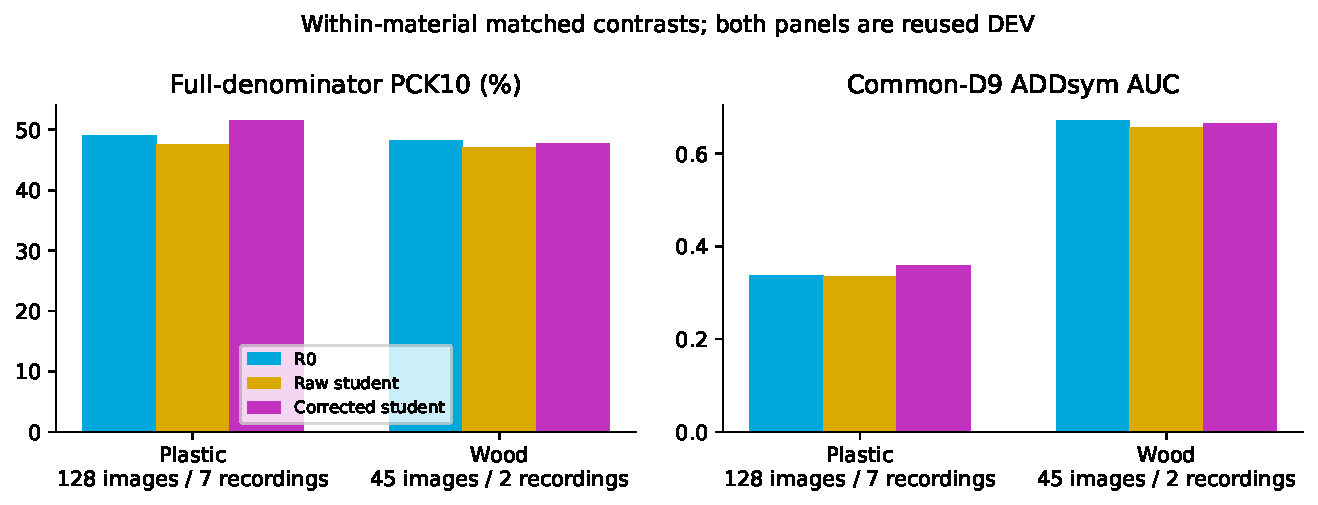
\includegraphics[width=.88\textwidth]{figures/material_main.pdf}
\caption{Material-stratified pooled results. Corrected-minus-raw PCK10 and common-D9 AUC are positive in both panels, but the wood effect is small and below R0. Absolute plastic/wood score differences combine different images, references, viewpoint distributions, and severity coverage; they do not isolate a causal material-difficulty effect.}
\label{fig:materials}
\end{figure*}

The prespecified pooled-direction decision is therefore \emph{material-general signal}, limited to the two evaluated categories. It is not evidence of material invariance, consistent gains in every recording, or verified wood pseudo-label quality. The historical material-routed experiments with type-specific teachers and Clean19 S0/S1/S2 used different supervision and interventions and remain supplementary context, not matched causal controls. The original plastic tables, LR/order sensitivity, verified66 tie, and bounded640-update study are preserved. No third option or further estimator experiment is introduced to enlarge this result.
